\documentclass[12pt]{article}
\usepackage[margin=1in]{geometry} 
\usepackage{amsmath,amsthm,amssymb,amsfonts,mathtools}
\usepackage{fancyhdr}
\usepackage{graphicx}
\graphicspath{ {./figures/} }

\newenvironment{problem}[2][]{
    \begin{trivlist}
        \item[
            {\bfseries #1}
            {\bfseries #2}
        ]
}{\end{trivlist}}

\newcommand{\chaptertitle}{Chapter 3 Motion in Two or Three Dimensions}
\newcommand{\sectiontitle}{\textsc{3.2 The Acceleration Vector}}
\newcommand{\name}{\textsc{Eric Nguyen}}

\pagestyle{fancy}
\chead{\sectiontitle \hfill \textsc{\today} \hfill \name}
\cfoot{\thepage}
\setlength{\headheight}{15pt}

\newcommand{\solution}{\medskip\noindent\textbf{Solution:}}
\newcommand{\Part}[1]{\shortintertext{(#1)}}
\newcommand{\PPart}[1]{\shortintertext{\qquad(#1)}}
\newcommand{\where}{, \, \text{ where }}
\newcommand{\magnitude}[1]{\lVert #1 \rVert}
\newcommand{\Vector}[2]{\langle #1, #2 \rangle}
\newcommand{\UVector}[2]{\left(#1\right)\ihat + \left(#2\right)\jhat}
\newcommand{\ihat}{\hat{\imath}}
\newcommand{\jhat}{\hat{\jmath}}
\newcommand{\radtodeg}[1]{\mbox{rad2deg}\left(#1\right)}

% UNITS
\newcommand{\unit}[1]{\, \text{#1}}

\newcommand{\cm}{\unit{cm}}
\newcommand{\m}{\unit{m}}
\newcommand{\km}{\unit{km}}
\newcommand{\ft}{\unit{ft}}
\newcommand{\inch}{\unit{in.}}
\newcommand{\mi}{\unit{mi}}
\newcommand{\gcm}{\unit{g/cm}}
\newcommand{\mum}{\, \mu \text{m}}
\newcommand{\mm}{\unit{mm}}

\newcommand{\Liter}{\unit{L}}
\newcommand{\gallon}{\unit{gallon}}
\newcommand{\kg}{\unit{kg}}
\newcommand{\g}{\unit{g}}
\newcommand{\lb}{\unit{lb}}

\newcommand{\mph}{\unit{mi/h}}
\newcommand{\kmh}{\unit{km/h}}
\newcommand{\kms}{\unit{km/s}}
\newcommand{\cms}{\unit{cm/s}}
\newcommand{\mps}{\unit{m/s}}
\newcommand{\mpg}{\unit{mpg}}
\newcommand{\kmL}{\unit{km/L}}

\newcommand{\y}{\unit{y}}
\newcommand{\mo}{\unit{mo}}
\newcommand{\ms}{\unit{ms}}
\newcommand{\ns}{\unit{ns}}
\newcommand{\s}{\unit{s}}
\newcommand{\gs}{\unit{gs}}
\newcommand{\days}{\unit{days}}
\newcommand{\Day}{\unit{day}}
\newcommand{\hours}{\unit{hrs}}
\newcommand{\hour}{\unit{hr}}
\newcommand{\Hour}{\unit{h}}
\newcommand{\minutes}{\unit{mins}}
\newcommand{\minute}{\unit{min}}

\newcommand{\ftpns}{\unit{ft/ns}}
\newcommand{\nspft}{\unit{ns/ft}}

\begin{document}

\begin{problem}{3.5}
    A jet plane is flying at a constant altitude.
    At time $t_1 = 0$, it has components of velocity $v_x = 90$ m/s, $v_y = 110$ m/s.
    At time $t_2 = 30.0$ s, the components are $v_x = -170$ m/s, $v_y = 40$ m/s.
    (a) Sketch the velocity vectors at $t_1$ and $t_2$.
    How do these two vectors differ?
    For this time interval calculate
    (b) the components of the average acceleration, and
    (c) the magnitude and direction of the average acceleration.

    \solution
    \begin{align*}
        &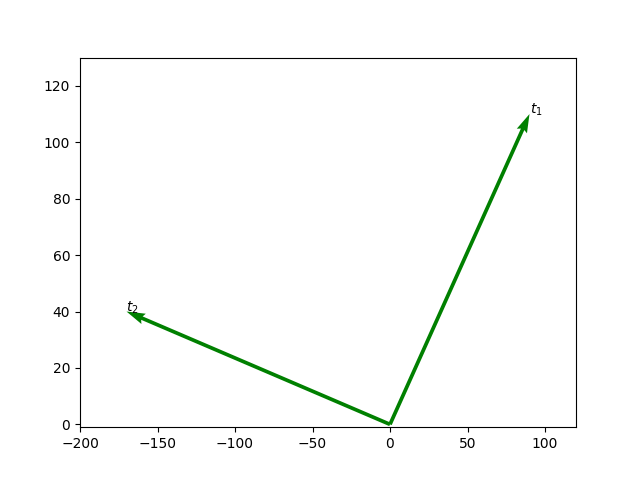
\includegraphics[scale=0.65]{3_05.png} \\
        &\text{The two vectors differ in their direction on the } x \text{-axis.}
    \end{align*}
    \begin{align}
        \vec{a}_{\text{av}} &= \frac{\Delta \vec{v}}{\Delta t} = \frac{\vec{v}_2 - \vec{v}_1}{t_2 - t_1} = \frac{\UVector{-170 \mps - 90 \mps}{40 \mps - 110 \mps}}{30.0 \s - 0} \\
        &= \frac{\UVector{-260 \mps}{70 \mps}}{30.0 \s} = \UVector{-\frac{26}{3} \mps^2}{-\frac{7}{3} \mps^2} \\
        \magnitude{\vec{a}_{\text{av}}} &= \sqrt{{\vec{a}_{\text{av-}x}}\phantom{}^2 + {\vec{a}_{\text{av-}y}}\phantom{}^2} = \sqrt{\left(-\frac{26}{3} \mps^2\right)^2 + \left(-\frac{7}{3} \mps^2\right)^2} \approx 8.98 \mps^2 \\
        \tan \beta &= \frac{\vec{a}_{\text{av-}y}}{\vec{a}_{\text{av-}x}} \Rightarrow \beta = 180^\circ + \radtodeg{\arctan\left(\frac{-\frac{7}{3} \mps^2}{-\frac{26}{3} \mps^2}\right) \mps^2} \approx 195^\circ
    \end{align}
\end{problem}

\clearpage

\begin{problem}{3.7}
    The coordinates of a bird flying in the $xy$-plane are given by $x(t) = \alpha t$ and $y(t) = 3.0 \m - \beta t^2$, where $\alpha = 2.4 \mps$ and $\beta = 1.2 \mps^2$.
    (a) Sketch the path of the bird between $t = 0$ and $t = 2.0 \s$.
    (b) Calculate the velocity and acceleration vectors of the bird as functions of time.
    (c) Calculate the magnitude and direction of the bird's velocity and acceleration at $t = 2.0 \s$.
    (d) Sketch the velocity and acceleration vectors at $t = 2.0 \s$. At this instant, is the bird's speed increasing, decreasing, or not changing?
    Is the bird turning?
    If so, in what direction?

    \solution
    \begin{align*}
        \Part{a}
        &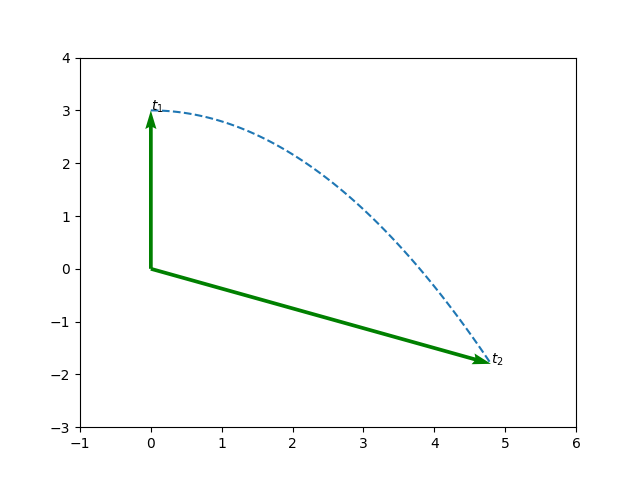
\includegraphics[scale=0.65]{3_07_a.png}
    \end{align*}
    \begin{align}
        \Part{b}
        \vec{r} &= \UVector{x(t)}{y(t)} \\
        \vec{v} &= \UVector{x'(t)}{y'(t)} \\
        &= \UVector{\alpha}{-2 \beta t} \\
        \vec{a} &= \UVector{x''(t)}{y''(t)} \\
        &= \UVector{0}{-2 \beta}
    \end{align}
    \begin{align}
        \Part{c}
        \magnitude{\vec{v}} &= \sqrt{\left(2.4 \mps\right)^2 + \left(-2 \left(1.2 \mps^2\right) \left(2.0 \s\right)\right)^2} \approx 5.4 \mps \\
        \alpha &= \radtodeg{\arctan{\left(\frac{-2 \left(1.2 \mps^2\right) \left(2.0 \s\right)}{\left(2.4 \mps\right)}\right)}} + 360^\circ \approx 297^\circ \\
        \magnitude{\vec{a}} &= -2 \left(1.2 \mps^2\right) \approx -2.4 \mps^2 \\
        \beta &= \radtodeg{\arctan\left(\frac{\left(-2.4 \mps^2\right)}{0}\right)} + 180^\circ = 270^\circ
    \end{align}
    \begin{align*}
        \Part{d}
        &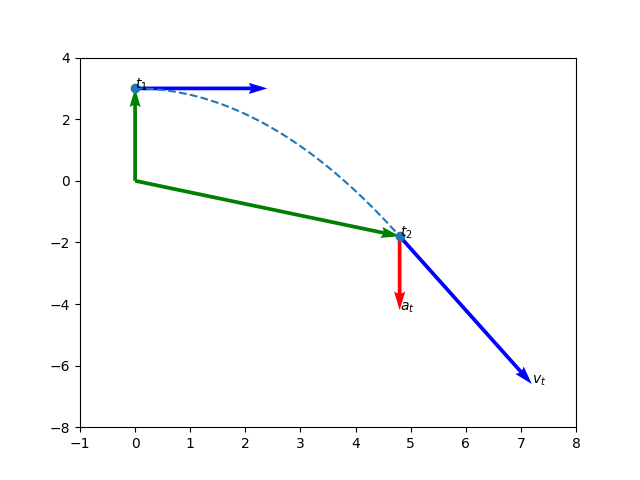
\includegraphics[scale=0.65]{3_07_d.png} 
    \end{align*}
    \begin{align}
        &\text{At this instant, where $t = 2.0 \s$, the bird's speed is increasing and is turning right.} 
    \end{align}
\end{problem}

\end{document}

